%!TEX root = Constructive Alignment for Introductory Programming.tex

\chapter{A Model for Constructively Aligned Introductory Programming} % (fold)
\label{cha:approach}

\graphicspath{{Figures/CAApproach/}}

\cref{cha:guiding_principles} outlined nine principles for guiding \emph{how} to teach introductory programming, and three principles for \emph{what} should be taught. This chapter proposes a model for applying constructive alignment for teaching introductory programming.

\section{Overall Strategy} % (fold)
\label{sec:overall_strategy}

One of the overarching principles from \cref{cha:guiding_principles} is the requirement to be agile and willing to change (\pref{itm:agile}). In discussing this principle, \sref{ssub:be_agile_and_willing_to_change} outlines that teaching and learning resources need to be guided by an overall strategy. This strategy informs, and is shaped by, the assessment approach and approach to the unit content.

This section first outlines the assessment approach, and then presents the approach this work took to delivering unit content. The decisions on which assessment approach was informed by the principles related to \emph{how} the teaching and learning environment should operate, while the approach to unit content is informed by the principles related to \emph{what} should be covered.

\subsection{Assessment Approach} % (fold)
\label{sub:assessment_approach}

Assessment plays an important role in defining what students learn. \citet{Rowntree:1977} indicated the central role of assessment procedures in understanding any education system. This is supported by \citet{Ramsden:2003}, who stated that ``from our students' point of view, assessment always defines the actual curriculum'', and further supported by \citet{Biggs:2007} who indicated that ``students learn what they \emph{thing} they will be tested on''. In presenting their conditions for effective assessment, \citet{Gibbs:2004} discussed the dominant influence of assessment in defining what students focus on, indicating that students are able to distinguish between what assessment requires them to pay attention to and what is likely to result in effective learning. So the selection of an assessment approach will have a significant impact on the overall strategy for both students and staff. 

Traditionally introductory programming was taught using a number of assignments and a final examination. This approach, while commonly used, is not in keeping with several of our guiding principles. The use of summative assessment during the semester goes against \pref{itm:formative} with its goal of assessing outcomes. The use of assignments to motivate students is also contrary to \pref{itm:theory_y}, with marks being used for motivation in either a hard or soft form of Theory X strategy. These principles required us to examine other forms of assessment.

One strategy to address this would be to consider abandoning coursework assignments, delay final summative assessment to an examination worth 100\% of the student's grade. While this would address \pref{itm:formative}, such a heavy weight examination is very much a hard Theory X approach. The value of coursework assignments was strongly argued for in \citet{Gibbs:2004}. This work provided several strong arguments for coursework assignments, including the following:
\begin{itemize}[noitemsep,nolistsep]
	\item Students attain better results from coursework than examinations, referring to their Gibbs' earlier work that indicated a strong positive correlation between proportion of coursework and average marks.
	\item Students prefer coursework assignments over examinations. A position that is supported by \citet{Kniveton:1996} who stated that students prefer coursework assignments to exams as assignments assessed a better range of their abilities and enabled them to organise their time to a greater extent.
	\item Coursework assignments are at least as valid a form of assessment as examinations:
	\begin{itemize}
		\item Exams are a poor predictor of future performance.
		\item Coursework assignments are a better predictor of long term learning than exam results \cite{Conway:1992}. This supports the idea that students adopt surface approaches to preparing for exams \citet{Marton:1976a}. 
		\item The quality of learning is higher in assignment-based units, when compared to exam-based units.
	\end{itemize}
\end{itemize}

The challenge, therefore, is to define an assessment approach that enables students to construct their knowledge, uses coursework assignments in a formative manner, and enables 100\% of the students grade to be determined after the end of the teaching period.

\subsubsection{Portfolio Assessment} % (fold)
\label{sub:portfolio_assessment}

In proposing Constructive Alignment, \citet{Biggs:1996c} advocated strongly for the use of an assessment portfolio, and indicated that the principles of constructive alignment had evolved with the decision to use portfolio assessment. This work was extended in \cite{Biggs:1997} which outlined suggestions for implementing portfolio assessment and a generalised model for instruction design. Further advice and details of the generalised model were presented in \citet{Biggs:2007} text on quality learning at university.

Assessment involves three components, all of which are typically under the control of the teacher \cite{Biggs:1997}. These include \emph{setting criteria}, \emph{selecting evidence} and \emph{making a judgement}. With the assessment portfolio the students take control of at least the selection of evidence. The portfolio is then a collection of work that the student puts forward for assessment against the unit's intended learning outcomes.

\citet{Smith:2001,Smith:2003} identified four different kinds of portfolios evident in the research literature: dossier, reflective, training and personal development. These reflected the combination of two factors: the purpose of the portfolio as either for selection/promotion or learning, and whether the portfolio is self-directed or mandated. The details of these are described in the following list, and shown in \fref{fig:portfolio_types}.

\begin{description}[noitemsep,nolistsep]
	\item[Dossier] is a portfolio for the purpose of selection or promotion that contains a mandated collection of work to demonstrate achievement. (selection/promotion, mandated)
	\item[Reflective] portfolios contain a self selected collection of work that demonstrates growth or accomplishment for the purpose of admission or promotion. The portfolio is accompanied by a self-appraisal, with the justification for the selection of pieces being as important as the evidence itself. (selection/promotion, self-directed)
	\item[Training] portfolios are a mandated collection of work performed in a learning context. The portfolio has a fixed format, and contains representative work from the student demonstrating acquired skills, knowledge and competencies. (learning, mandated)
	\item[Personal development] portfolios are a self selected collection of work, and reflective account of personal growth over an extended period. (learning, self-directed)
\end{description}

\begin{figure}[htbp]
	\centering
	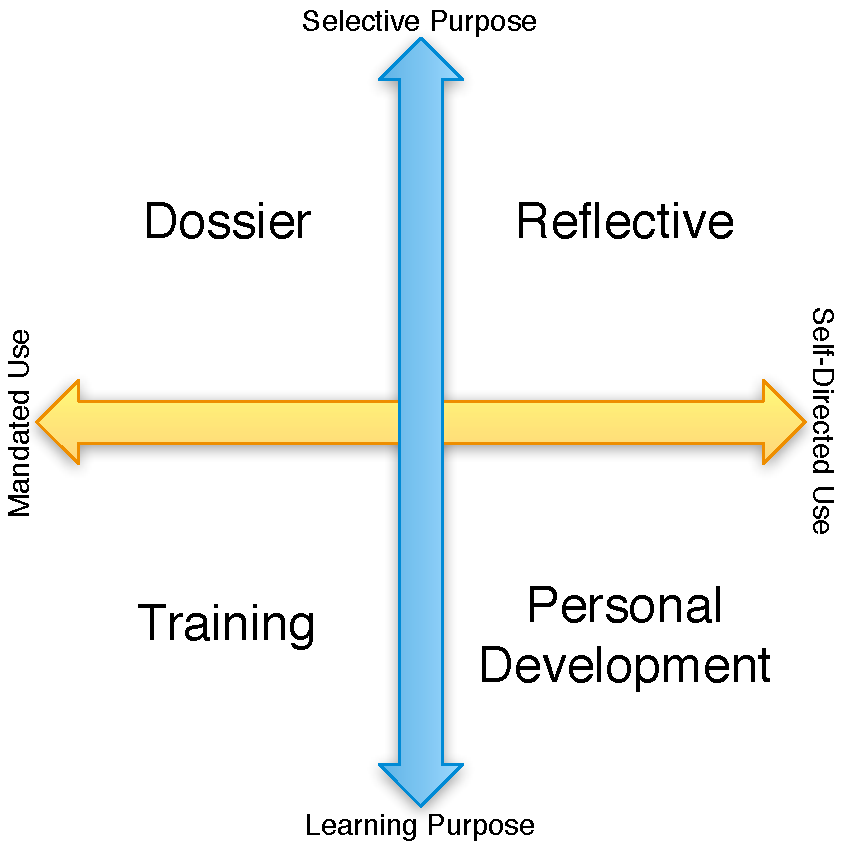
\includegraphics[width=0.50\textwidth]{PortfolioTypes}
	\caption{The four kinds of portfolio based upon purpose and use from \citet{Smith:2001}.}
	\label{fig:portfolio_types}
\end{figure}

Biggs' use of an \emph{assessment portfolio} clearly fits with the \emph{Training} portfolio classification, being a mandated part of the unit assessment for the purpose of evaluating learning outcomes. In the study of a small group of professionals, \citet{Smith:2001} found the training portfolio to be highly rated. Their findings indicated that students found the training portfolio confusing initially, but that once they had understood its function and rational they liked the approach, were easily able to construct their portfolio, and felt it was a fair way to assess their learning.

\citet{Tang:1999} provides further evidence of the value of portfolio assessment. In evaluating how students approach study, \citet{Tang:1999} found that students tended to have a narrow, surface approach to studying for tests. These same students were found to adopt wider, more cognitively challenging, approaches when preparing for a portfolio assessment. 

Portfolio assessment enables the shift from Theory X ``sage on the stage'' views to a Theory Y ``guide by the side'' view. The traditional approach of setting assignments and exams in which educators test student ability becomes inverted with portfolio assessment. With portfolio assessment it is the students responsibility to demonstrate how they have met the unit's intended learning outcomes. This frees educators to help students and to guide them in the preparation of their evidence. We are now working side by side with the students, helping them to achieve the intended learning outcomes.

Portfolio assessment appears to align well with all nine ``\emph{how}'' principles listed in \cref{cha:guiding_principles}. 
\begin{itemize}[noitemsep,nolistsep]
	\item The portfolio consists of a collection of work the student feels demonstrates the depth of their knowledge. (\Pref{itm:construct})
	\item Assessment criteria for the portfolio can be aligned with the unit's intended learning outcomes. (\Pref{itm:align})
	\item The portfolio can be used as the sole form of summative assessment, with students being able to take advantage of formative feedback throughout the teaching period. (\Pref{itm:formative})
	\item A focus on depth will ensure the portfolio requires students to engage high cognitive levels, requiring them to explain, justify and reflect. (\Pref{itm:depth})
	\item By communicating high expectations, students will strive to create high quality evidence for their portfolios. (\Pref{itm:expectations})
	\item Students will develop evidence for their portfolio from day 1, everything they do could be of potential value. This will require active support from teaching staff. (\Pref{itm:support})
	\item Without marks for motivation, an entirely portfolio assessed unit empowers students in the learning process, and must trust that they are able to effectively manage their own learning. (\Pref{itm:theory_y})
	\item Portfolio assessment, with frequent formative feedback, is very much akin to agile software development processes. In addition, student portfolios will provide a wealth of evidence to help guide change. (\Pref{itm:agile})
	\item Incorporating a reflective component in the portfolio will encourage students to engage in reflective practice. (\Pref{itm:reflect})
\end{itemize}

Given its role in the formation of constructive alignment and its clear alignment with the principles, the approach to constructively aligned introductory programming presented in this chapter uses portfolio assessment.

A number of papers have discussed portfolio assessment for introductory programming units. \cite{Plimmer:2000} reported the successful use of portfolio assessment in an introductory programming unit in which the portfolio contributed between 25\% and 60\% of the students' final grades. Programming portfolios were also discussed by \cite{Jones:2010}, where students submitted a number of portfolio assignments during the semester. In both cases the portfolio was a collection of programs that were marked and contributed to a final grade, rather than being used as a holistic assessment of the student's ability to meet the intended learning outcomes, as is the case with portfolio assessment in our approach to constructive alignment. 


% subsection portfolio_assessment (end)
% subsection assessment_approach (end)

\subsection{Content Approach} % (fold)
\label{sub:content_approach}

The second aspect of the overall strategy is to define an approach for selecting unit content. \sref{sec:principles_to_guide_what_we_should_cover} presented a number of principles related to what should be taught in introductory programming, with \pref{itm:paradigm} indicating that the overall strategy needs to be defined around a programming paradigm. This section addresses the question of which programming paradigms were selected for introductory programming in this work.

Prior to conducting this research we have experienced introductory programming using both imperative-first and objects-first approaches. Our view mirrors those of \citet{Rist:1996} who reported on plans and cognitive schemas, the fundamental units of program design. In relating plans to objects, \citet{Rist:1996} indicated that objects were not different, they were more, as objects require additional overhead related to defining object\footnote{Object structures are typically defined using classes or similar mechanisms in languages such as Java} structures. Given this, units that take an objects-first approach will still need to have a significant focus on procedural aspects, as indicated by \citet{Robins:2003}. This reasoning was echoed in the ``back to basics'' approach from \citet{Reges:2006}.

\pref{itm:depth} indicates that in this work we aim to build a depth of knowledge, over breadth of coverage. If, as \citet{Rist:1996} claimed, objects are ``more'' then our principles indicate that an objects-later approach should be taken. This is further supported by the 2013 Computer Science Curricula \cite{CSC2013}, which listed primarily imperative programming concepts in its section on Software Development Fundamentals.

An objects-later approach also matches the concept-based approach outlined in \cref{cha:guiding_principles}. \pref{itm:concepts} indicates a focus on programming concepts, which are built on top of previously covered concepts to enable students to explore the language, and programming in general. By starting with imperative programming the unit can start with fundamental concepts, and work up to the concept of objects.

\citet{Reges:2006} back to basics approach taught imperative programming concepts using the Java programming language. Java is an object oriented programming language, and so in effect this approach taught students how \emph{not} to use Java. While we will adopt the imperative programming focus, \pref{itm:authentic} indicates that we must select a programming language that was designed for this purpose. The language choice is discussed in \cref{cha:example_impl}.

While objects would not appear in the first programming unit, their importance in students' education remained a focus. Rather than seeing programming as being delivered in a single stand alone unit, we designed a sequence of two units that worked closely together. The first covered structured procedural programming, focusing on aspects such as control flow. The second focused on object oriented programming, which can then use a model driven approach similar to the one reported in \citet{Bennedsen:2004} but without having to cover procedural programming aspects such as control flow.

Given its focus on fundamentals, an objects-later approach was used in the curriculum presented in this work. This aligns well with the principles in \cref{cha:guiding_principles} with its focus on depth over breadth, and its ability to match the proposed concept-based approach to introductory programming. Object oriented programming was then the content of a second programming unit. The alignment of these two units to the \emph{what} principles from \cref{cha:guiding_principles} is outlined in the following list.
\begin{enumerate}[noitemsep,nolistsep]
	\item The first programming unit, introductory programming, aligned with the principles in the following way:
	\begin{itemize}[noitemsep,nolistsep]
		\item Content selection was guided by the structured procedural programming paradigm.
		\item Focus will be on fundamental programming concepts, which included functions and procedures, variables, control flow, parameter passing, etcetera.
		\item The chosen programming language, or languages, must have been designed for procedural programming.
	\end{itemize}
	\item The second programming unit, object oriented programming, aligned with the principles in the following way:
	\begin{itemize}[noitemsep,nolistsep]
		\item Content selection was guided by the object oriented programming paradigm.
		\item Focus will be on object oriented programming concepts including abstraction, encapsulation, inheritance and polymorphism, etcetera.
		\item The chosen programming language, or languages, must have been designed for object oriented programming.
	\end{itemize}
\end{enumerate}



% subsection content_approach (end)

\subsection{Summary} % (fold)
\label{sub:summary}

The overall strategy is defined by two approaches: the assessment approach, and the approach to content selection. Decisions related to these two approach were guided by the principles from \cref{cha:guiding_principles}, and resulted in the selection of a \textbf{portfolio assessment} approach to units that are taught using an \textbf{objects-later} approach to content selection. \fref{fig:overall_strategy} shows an updated version of \fref{fig:strategy}, showing the selected approaches discussed in this section. The next section describes the model for constructively aligned introductory programming that developed from this overall strategy.

\begin{figure}[p]
	\centering
	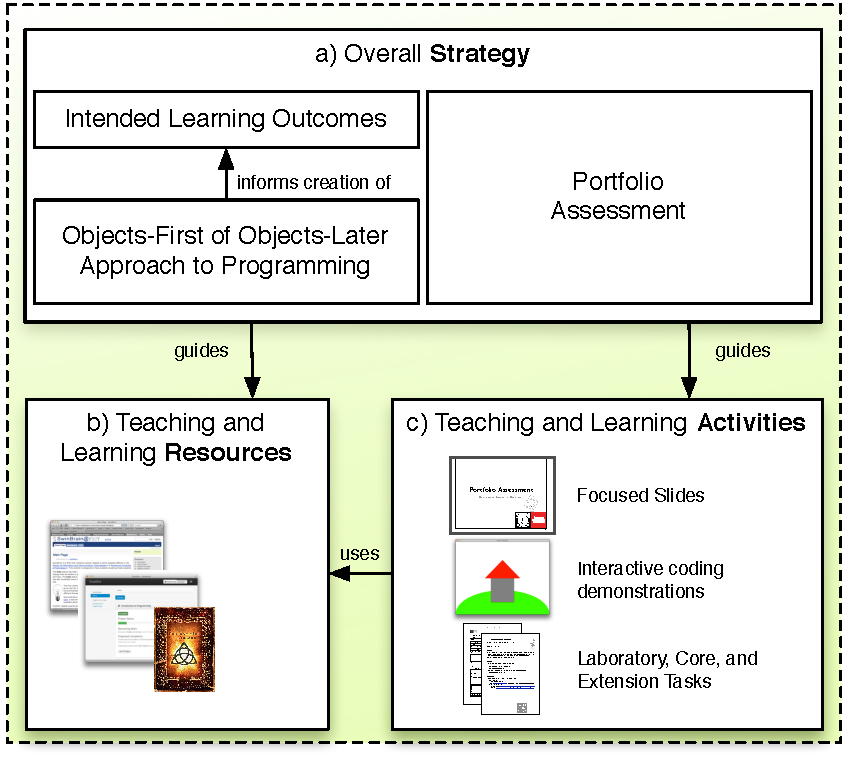
\includegraphics[width=\textwidth]{OverallStrategy}
	\caption{An updated version of \fref{fig:strategy} showing the selected assessment approach, and the programming paradigms that will form the approach for selecting content.}
	\label{fig:overall_strategy}
\end{figure}

% subsection summary (end)
% section overall_strategy (end)

\clearpage
\section{Constructively Aligned Introductory Programming} % (fold)
\label{sec:model}

\subsection{Model Overview} % (fold)
\label{sub:model_overview}

Having decided upon an overall strategy, the next stage of our research was to determine how Biggs' model of constructive alignment~\cite{Biggs:1996c}, and the details on using portfolio assessment suggested by \citet{Biggs:1997}, could be used to guide the creation of an introductory programming unit. This involved the examination of the practical advice from \citet{Biggs:2007}, which further elaborates on Biggs' model of constructive alignment and portfolio assessment. Using this together with the principles from \cref{cha:guiding_principles}, a model of constructive alignment for introductory programming was defined. The resulting model was documented in \citet{Cain:2012a}, and captured staff and student processes and the artefacts generated and exchanged throughout the learning process, as illustrated in \fref{fig:process_overview}.

\begin{figure}[htbp]
	\centering
	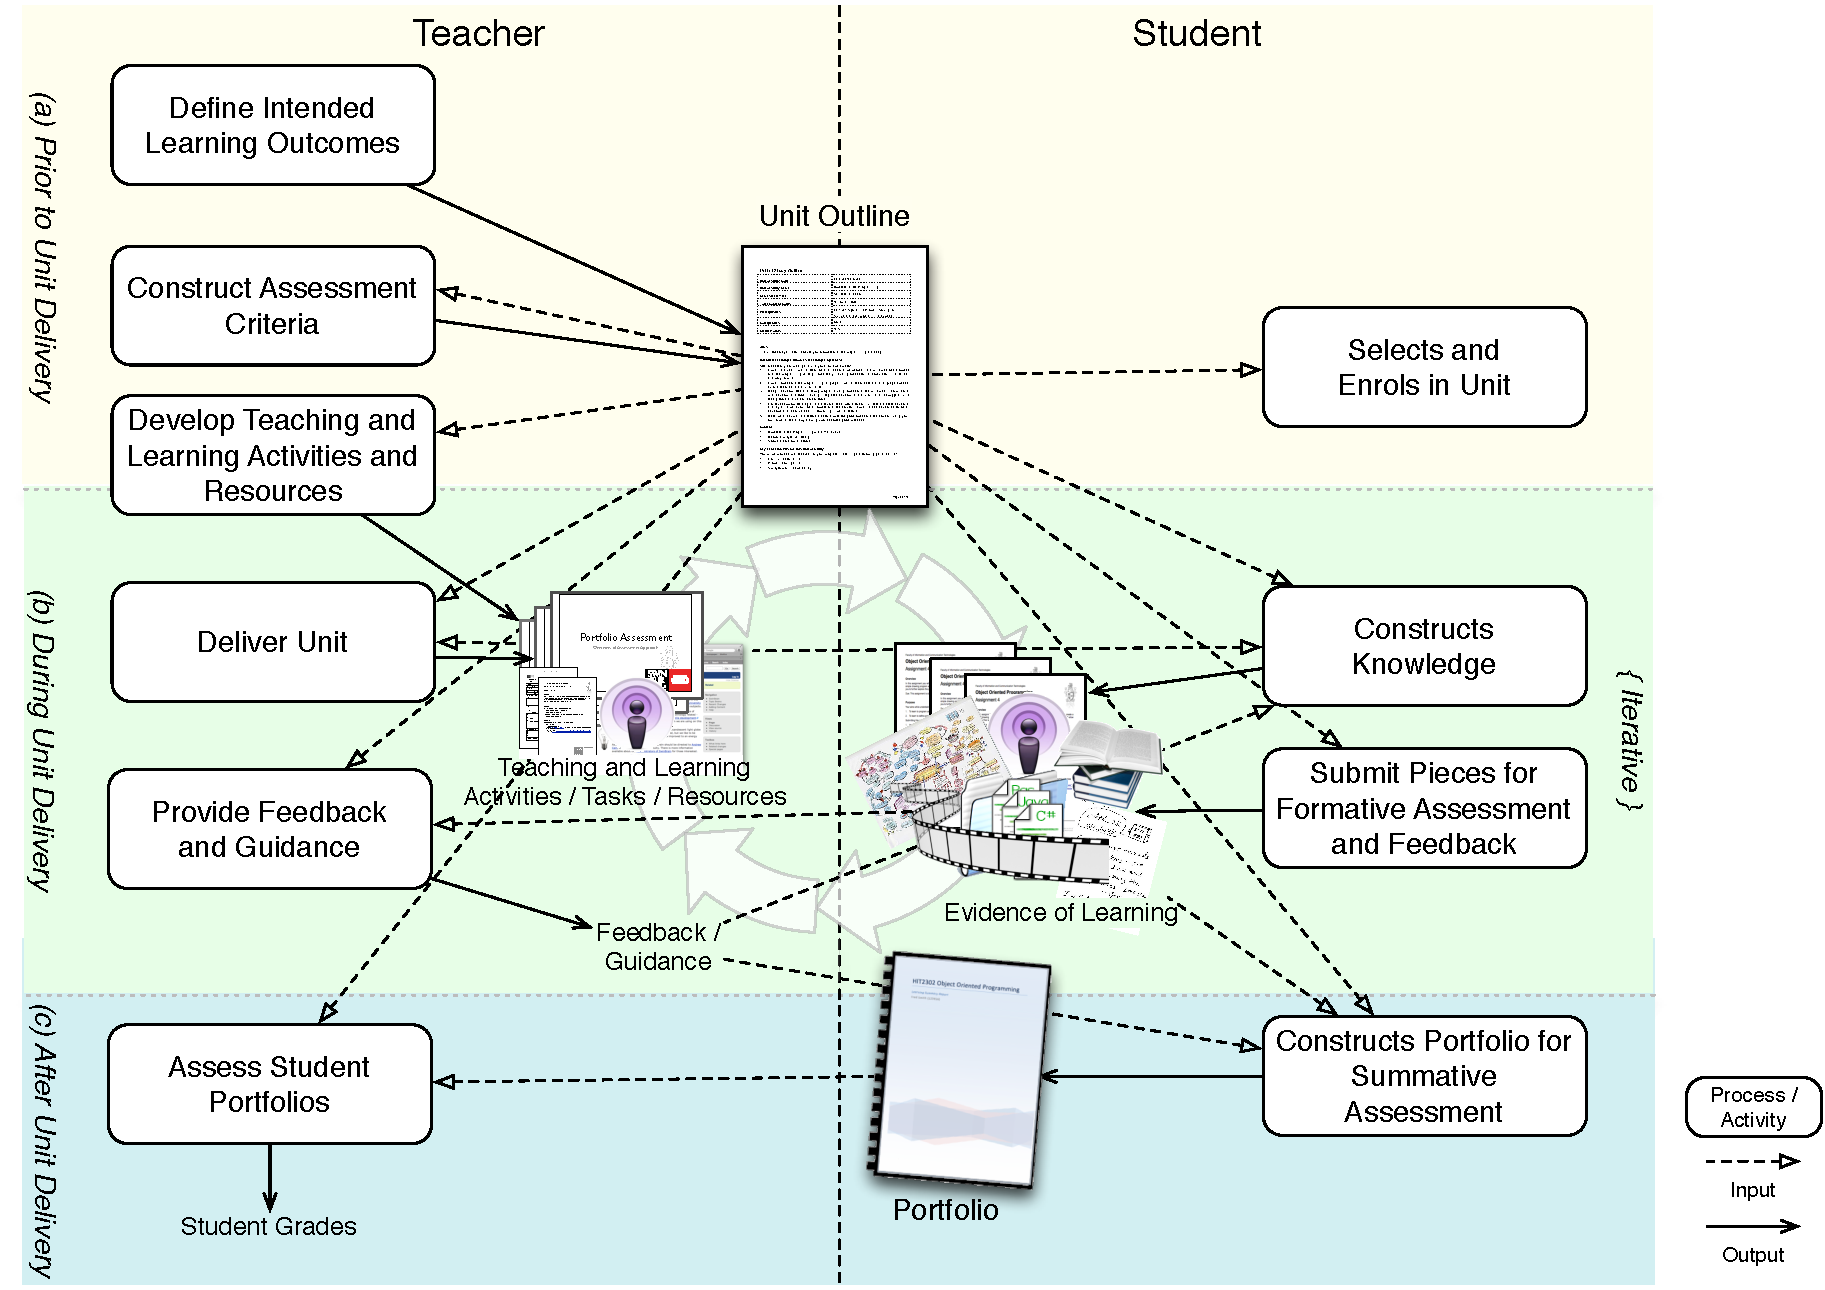
\includegraphics[width=\textwidth]{ProcessOverview}
	\caption{An overview of teacher and students roles, and iterative delivery, in the constructive alignment model developed for introductory programming.}
	\label{fig:process_overview}
\end{figure}

Processes within the model are performed either by \emph{students} or \emph{teaching staff}. These processes are distributed across three stages of unit development and delivery: being either \emph{prior} to the start of the teaching period, \emph{during} the teaching period, or \emph{after} the teaching period. \fref{fig:process_overview} illustrates this with separate columns for teaching and student processes, and rows for the stages in which these processes occur.

Prior to the start of the teaching period (a) the teaching staff \emph{define intended learning outcomes} and \emph{construct assessment criteria}. Together these aspects form a critical component of unit, defining what students will be able to achieve after successfully completing the unit, and how well they must perform in order to achieve different grade outcomes. Both the intended learning outcomes and assessment criteria are documented in the Unit Outline, a document that is a common practice in university environments. The Unit Outline forms the central focus for subsequent processes, and informs and guides staff in the \emph{development of teaching and learning activities}. Unit outlines may also be used by students in evaluating units to select in their course of study.

The developed teaching and learning activities and their associated resources are then used during the teaching period (b) by staff to \emph{deliver the unit}. Students follow the guidance of teaching staff, and ideally these activities aid students as they \emph{construct knowledge}. The work that students produce can then be \emph{submitted for formative feedback}, which provides an opportunity for teaching staff to \emph{provide feedback and guidance}. The process of students undertaking activities, constructing knowledge, and receiving formative feedback is designed to be an ongoing iterative process throughout the teaching period.

After the conclusion of the teaching period (c) students prepare their work for summative assessment through the \emph{construction and submission of their portfolios}. These portfolios are then \emph{assessed by} the teaching staff against the intended learning outcomes and assessment criteria prepared prior to the unit's delivery.

Each of these processes is described in more detail in the following section.

% subsection model_overview (end)

\subsection{Processes within the Model} % (fold)
\label{sub:processes_within_the_model}

\subsubsection{Defining Intended Learning Outcomes} % (fold)
\label{sub:defining_intended_learning_outcomes}

Intended learning outcomes are central to the concept of constructive alignment as a statement of what students will be able to achieve at the end of the unit. Aligned curriculum in constructive alignment indicates that teaching and learning activities and assessment must \emph{align} to these intended learning outcomes. The findings in \cref{cha:background} indicate that alignment is typically performed by staff who indicate how teaching and learning activities and assessment tasks are aligned. Alignment is a matter external from the actual teaching itself. There is little involvement of the student in this process.

With portfolio assessment the alignment becomes intrinsically entwined with unit delivery and assessment. The teaching staff relinquish control of this aspect and the outcomes themselves take on their true purpose: as a statement of what students will be able to achieve at the end of the unit. All other aspects of the unit must now align to this purpose. Teaching and learning activities must prepare students to demonstrate that they have achieve these outcomes. Assessment aims to verify the extent to which students have reached these outcomes.

One way to conceptualise the central role of the intended learning outcomes is to picture this situation as a very long examination. The intended learning outcomes are the questions, the things students need to demonstrate they can do by the end of the ``exam''. The intended learning outcomes have become the assessment, a direct realisation of the fact that ``assessment always drives the curriculum'' \cite{Ramsden:2003}.  In this arrangement there is little opportunity for misalignment between the unit objectives and assessment, but a greater importance on the exact nature of the intended learning outcomes. This critical role of the intended learning outcomes means that they are instrumental in the success of the unit. 

For the introductory programming units it was important to design the intended learning outcomes so that, as a group, they cover the required programming competencies as well as the associated conceptual knowledge. The intended learning outcomes play a central role in driving the processes of both students and teaching staff. As a result, it is important they are expressed clearly and simply so as to be understood by all involved.

Development of unit outcomes has a variety of input sources, as shown in \fref{fig:defining_ilos}. \citet{Thota:2010} propose inputs related to pedagogic theory (constructivism and phenomenography) as well as student factors such as approach to learning, learning styles, and prior knowledge. \citet{Armarego:2009} highlights the needs for inputs from industry, such as the Computer Science and Software Engineering Curriculum from professional standards bodies (see \citet{Lethbridge:2006}, \citet{Cassel:2008} and \citet{CSC2013}), and associated Bodies of Knowledge (see \citet{Abran:2001}). 

In addition to these sources we included the guiding principles and overall strategy, as well as resourcing factors and accreditation requirements. Resourcing factors provide additional constraints on what intended learning outcomes can include. Factors such as staffing, availability of texts, required tools, etcetera all need to be considered to ensure that students will be able to engage in activities associated with demonstrating the expected outcomes. Accreditation standards, such as the Australian Qualifications Framework \cite{AQF:2013}, require intended learning outcomes to demonstrate certain levels of achievement in order for courses to gain recognition and funding. As these units will form an important part of course objectives, these requirements must also be considered. 

\begin{figure}[htbp]
	\centering
	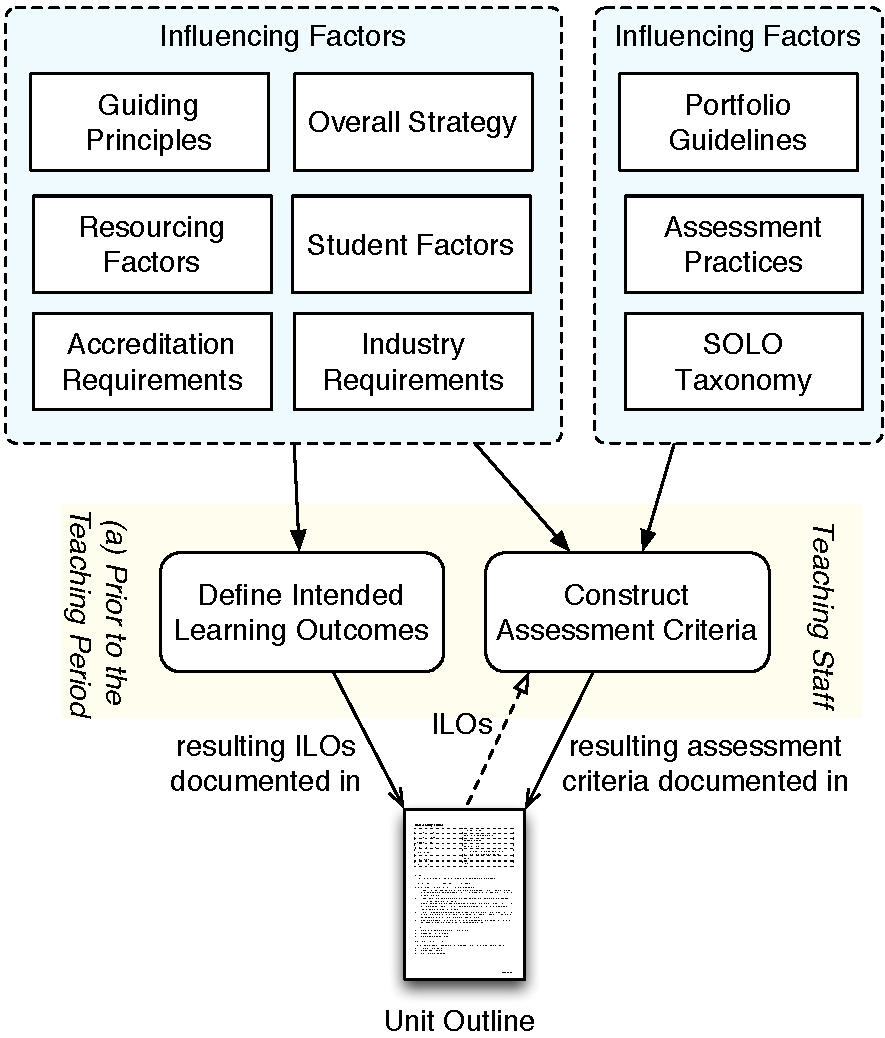
\includegraphics[width=0.7\textwidth]{DefiningILOs}
	\caption{Factors that influence the defining of a unit's intended learning outcomes, and the construction of assessment criteria.}
	\label{fig:defining_ilos}
\end{figure}

\citet{Biggs:2007} provided a number of recommendations for the development of intended learning outcomes. They indicated that it was appropriate for a unit to have between four and six intended learning outcomes, expressed at suitably high cognitive levels. Adopting this approach enables the focus on depth over breadth, \pref{itm:depth} from \cref{cha:guiding_principles}. A small number of intended learning outcomes keep the focus clear for students.

% removed SOLO details from here...

The SOLO Taxonomy proposed by \citet{Biggs:1982} provides a framework for ensuring intended learning outcomes aim for suitably high cognitive levels. Each of the identified cognitive levels has an associated list of verbs likely to elicit that level of activity. \tref{tbl:solo_verbs} lists verbs associated with the various levels of the SOLO taxonomy. These verbs can be used when defining the unit's intended learning outcomes. Biggs suggests that intended learning outcomes for university level units should aim for at least the multistructural level, with many units aiming for understanding at the relational level. In a review of science curricula in Danish universities, \citet{Brabrand:2009} argued that the SOLO taxonomy provided a good tool for competency with a range of areas showing progressing in terms of SOLO verbs from undergraduate to graduate education.

\begin{table}
	\renewcommand{\arraystretch}{1.6}
	\centering
	\caption{Selected list of verb related to the various levels of the SOLO Taxonomy, adapted from \citet{Biggs:2007}}
 	\label{tbl:solo_verbs}

    \begin{tabular}{lp{10cm}}
    SOLO Level        & Verbs \\
    \hline
    \textbf{Unistructural}     & Memorize, identify, recognise, count, define, draw, find, label, match, name, quote, recall, recite, order, tell, write, imitate\\
    \textbf{Multistructural}   & Classify, describe, list, report, discuss, illustrate, select, narrate, compute, sequence, outline, separate\\
    \textbf{Relational}        & Apply, integrate, analyse, explain, predict, conclude, summarise, review, argue, transfer, plan, characterise, compare, contrast, differentiate, organise, debate, make a case, construct, review and rewrite, examine, translate, paraphrase, explain causes \\
    \textbf{Extended Abstract} & Theorise, hypothesise, generalise, invent, originate, make original case\\
    \end{tabular}
\end{table}

\clearpage
We developed the following principles which can be used to guide the formation of the intended learning outcomes for portfolio assessed programming units:
\begin{itemize}[noitemsep,nolistsep]
  \item Express outcomes using verbs at an appropriate level of understanding with reference to the SOLO taxonomy.
  \item Cover both the required \emph{conceptual knowledge}, and \emph{programming competencies}.
  \item Use \emph{simple terms} (where possible) to communicate outcomes, ensuring they are understood by all students undertaking the unit.
  \item The number of outcomes should be \emph{minimal}, ideally between four and six. This is to help ensure that each outcome covers a meaningful body of knowledge to a sufficient depth.
  \item Outcomes need to be \emph{general} to facilitate assessment of diverse portfolios, and \emph{sufficient} to ensure that differing degrees of proficiency and understanding can be assessed.
  \item There needs to be \emph{flexibility} to enable students to choose a range of means when addressing outcomes.
\end{itemize}

% subsection processes_within_the_model (end)
\subsubsection{Constructing Assessment Criteria} % (fold)
\label{sub:constructing_assessment_criteria}

Assessment criteria are developed alongside the definition of the intended learning outcomes. The intended learning outcomes state what students need to demonstrate by the end of the unit, but these outcomes can be achieved to different standards. It is the role of the assessment criteria to state the required level of achievement students must demonstrate in order to be awarded various grade outcomes. This means that at the end of the teaching period students portfolios can be assessed against using the developed assessment criteria, but also that the assessment criteria can be used to guide the teaching and learning activities during delivery. Providing assessment criteria in the unit outline creates a simplified learning contract \cite{Stephenson:1993}, in which students know ``up front'' what is required to achieve the different grades. 

\pref{itm:formative} indicates that assessment should judge outcomes.To provide this holistic judgement the final summative assessment is \emph{criterion-referenced}, as suggested by \citet{Biggs:1997}. The criteria must, therefore, provide a means for teaching staff to assess submitted portfolios while also providing students with guidance they can use during the delivery and in the construction of their portfolios. Ensuring that the assessment criteria are stated clearly will help ease students transition to this new form of assessment \cite{Smith:2001}.

There is some contention regarding the specification of assessment criteria for assessing portfolios. For example, some consider that by overly specifying criteria students are limited in what can be included (see \citet{Driessen:2005} and \citet{Tigelaar:2007}). 
However, \citet{Smith:2001} indicated that clearly communicating portfolio requirements helped ease students transition to this new assessment approach. \citet{Allan:1996} argued that clear communication of intended learning outcomes and assessment criteria, enables students to focus on developing knowledge required to succeed in a unit. \citet{Thorpe:2000} reported that students find it difficult to reflect on what they have learnt, and noted that this process is made easier for students if they apply criteria defined by teaching staff.

The assessment criteria development process takes input from the intended learning outcomes, along with guidelines for portfolio assessment \cite{Biggs:2007} and levels of achievement from the SOLO taxonomy \cite{Biggs:1982} as shown in \fref{fig:defining_ilos}. The resulting criteria are placed alongside the intended learning outcomes in the unit outline.

In order to facilitate assessment, and to guide student activity, the assessment criteria need to indicate clearly distinct requirements for each grade outcome. In the university where this work was carried out there are five grade categories: fail, pass, credit, distinction and high distinction. The assessment criteria indicate what students need to demonstrate to achieve each grade. 

The following list presents the assessment criteria developed in this work. The criteria are cumulative, with each level beyond pass requiring all previous requirements to be satisfied in addition to some deeper level of understanding being demonstrated. Pass requires that each intended learning outcome is met to a minimally acceptable standard, which will depend on the verb used in their description. Credit then requires an overall picture of the unit, with students starting to see how the various aspects of the unit come together as a whole. This is then required to achieve the Distinction grade, in which students must show they can apply unit concepts to the creation of a piece of work of their own invention. This does not need to be new or ground breaking work, just something they came up with that shows all of the intended learning outcomes in play. High Distinction then goes beyond this by asking students to engage is a small research project, encouraging them to work toward an extended abstract\footnote{Extended abstract requires a level of understanding where new knowledge can be created.} level of understanding, but not requiring that they achieve this.
\begin{description}[noitemsep,nolistsep]
	\item[Fail] is a result of anything less than Pass level.
	\item[Pass] demonstrates \emph{minimally acceptable} level of achievement. Students have been able to complete core tasks from the teaching and learning activities, and pass any hurdle\footnote{Hurdle requirements are anything that must be ``passed'' to pass the unit, but do not contribute marks toward the final grade.} requirements.
	\item[Credit] demonstrates all Pass requirements and shows a \emph{good} depth of understanding across all intended learning outcomes, but does not go beyond presented work. Demonstrates at least a multistructural level of understanding of the unit overall.
	\item[Distinction] demonstrates Credit level requirements and the ability to \emph{apply} unit concepts to the creation of work of the students own invention. This demonstrates at least a relational level of understanding of the unit overall.
	\item[High Distinction] demonstrates all Distinction level requirements and the ability to \emph{research} a topic related to the unit. This still requires only a relational level of understanding, but provides opportunities and encouragement for students to explore beyond the current knowledge and work toward that extended abstract level of understanding.
\end{description}

The following principles were used to guide the definition and communication of the assessment criteria:

\begin{itemize}[noitemsep,nolistsep]
  \item Communicate assessment criteria using \emph{simple terms} (as suggested for the outcomes).
  \item Require sufficient progress to be demonstrated for all intended learning outcomes. At least a multistructural level of understanding should be obtained for passing students.
  \item Higher grades should require:
  \begin{itemize}[noitemsep,nolistsep]
  	\item evidence of \emph{deeper learning}, while specifically avoiding an excessive volume of work.
  	\item integrated understanding across related intended learning outcomes, as well as within each intended learning outcome.
  \end{itemize}
  \item Aim to develop \emph{clearly distinct} assessment criteria for each grade outcome, facilitating timely assessment and providing clear requirements for students.  
  \item Clearly \emph{map assessment criteria} to grade outcomes, ensuring students and staff have a shared understanding of how a portfolio relates to final grades.
\end{itemize}


% section a_constructively_aligned_model_for_introductory_programming (end)

\subsubsection{Develop Teaching and Learning Activities and Resources} % (fold)
\label{ssub:develop_teaching_and_learning_activities_and_resources}

Having defined the intended learning outcome and assessment criteria, teaching staff develop, or select, appropriate teaching and learning activities and resources. \fref{fig:develop_tlar} illustrates the role of this process in the overall unit delivery. The process uses inputs from the Unit Outline, and generates both teaching and learning activities and resources.

\begin{figure}[htbp]
	\centering
	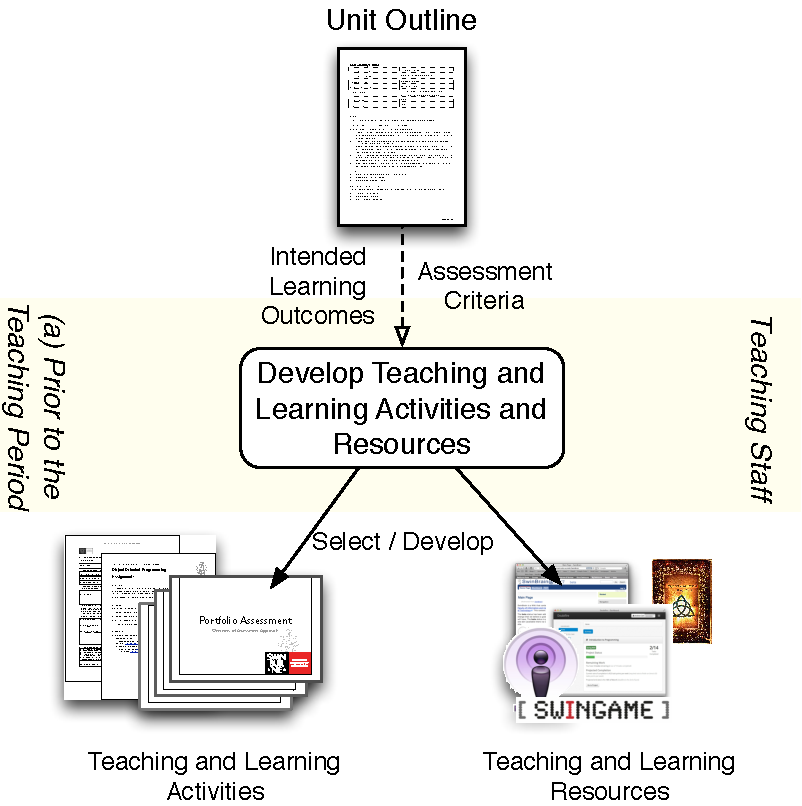
\includegraphics[width=0.8\textwidth]{DevelopTLAR}
	\caption{Development of teaching and learning activities and resources uses details from the unit outline to create/select appropriate resources and activities to ensure students engage appropriate activities during the teaching period.}
	\label{fig:develop_tlar}
\end{figure}

The teaching and learning activities aim to elicit appropriate behaviour from students, ensuring that they engage in the cognitive processes representative of the desired level of achievement for each intended learning outcome. Output generated from this process will include lecture slides and tutorial/laboratory handouts. In relation of the overall strategy, these activities are likely to change frequently as we are better able to direct student efforts. In keeping with our agile principles, \pref{itm:agile}, the effort spent on developing these should, therefore, be minimised.

Teaching and learning resources, on the other hand, provide students with the details they will require to successfully complete these activities. These resources will have longer lasting value, and can change less frequently than the teaching and learning activities. 

Central to this approach is the idea of focusing each aspect of the teaching and learning environment to best benefit the construction of student knowledge. Teaching and learning resources provide details, and extra attention and effort are required in their development with the benefit of being able to be used in a range of contexts. Examples of resources include textual and visual illustrations, video podcasts showing example usage, online tools, and supportive software. Some of these resources can then be used in the creation of the lecture slides, but the lectures focus on providing cognitive guidance, directing students through the most important aspects with the details to be discovered later when students make use of the provided resources.

The following principles were used to guide this process:
\begin{itemize}[noitemsep,nolistsep]
	\item Teaching and learning activities should:
	\begin{itemize}[noitemsep,nolistsep]
	 	\item Actively engage the students.
	 	\item Align with the unit's intended learning outcomes.
	 	\item Focus on providing guidance:
	 	\begin{itemize}[noitemsep,nolistsep]
		 	\item Lectures should inform, motivate and inspire students. Providing them with the key ingredients needed to get started with the tutorial/laboratory tasks.
		 	\item Tutorial/Laboratory tasks should direct students to perform activities that engage appropriate cognitive levels, helping them create artefacts that can be included in their portfolios.
	 	\end{itemize}
	 \end{itemize} 

	\item Teaching and learning resources should:
	\begin{itemize}[noitemsep,nolistsep]
		\item Provide the details students require to perform the tasks from the teaching and learning activities.
		\item Be created with a focus on re-usability.
		\item Support a range of different learning styles.
	\end{itemize}
\end{itemize}

% subsubsection develop_teaching_and_learning_activities_and_resources (end)

\subsubsection{Iteratively Deliver Unit and Provide Feedback} % (fold)
\label{ssub:deliver_unit}

Constructive learning theories emphasise the active role of the learner in constructing knowledge. Our guiding principles are centred on this notion and adopt Biggs' pragmatic view of constructivism. The iterative, students centred, delivery process aims to embody Biggs' quote ``It's what the student does that counts.'' \cite{Biggs:1996c}, a statement that can be traced back to Tyler's quote, ``It is what he does that he learns, not what the teacher does'' \cite{Tyler:1969}.

Existing work on constructive approaches to teaching introductory programming provide some advice on designing and delivering student-centred teaching and learning activities. \citet{BenAri:1998,BenAri:2001} discussed the need for students to construct appropriate models of the computer. \citet{VanGorp:2001} described collaborative and constructive environments with the use of code walk-throughs, writing code, debugging and other activities. \citet{Thramboulidis:2003} presented a design first approach to object oriented programming that focused on engaging students with object oriented design processes. \citet{Wulf:2005} reported strategies such as moving content from lectures to online video presentations. Similarly, the work of \citet{Thota:2010} also presented constructive approaches to teaching introductory programming that focused on group work, and the active role of the student.

\begin{figure}[p]
	\centering
	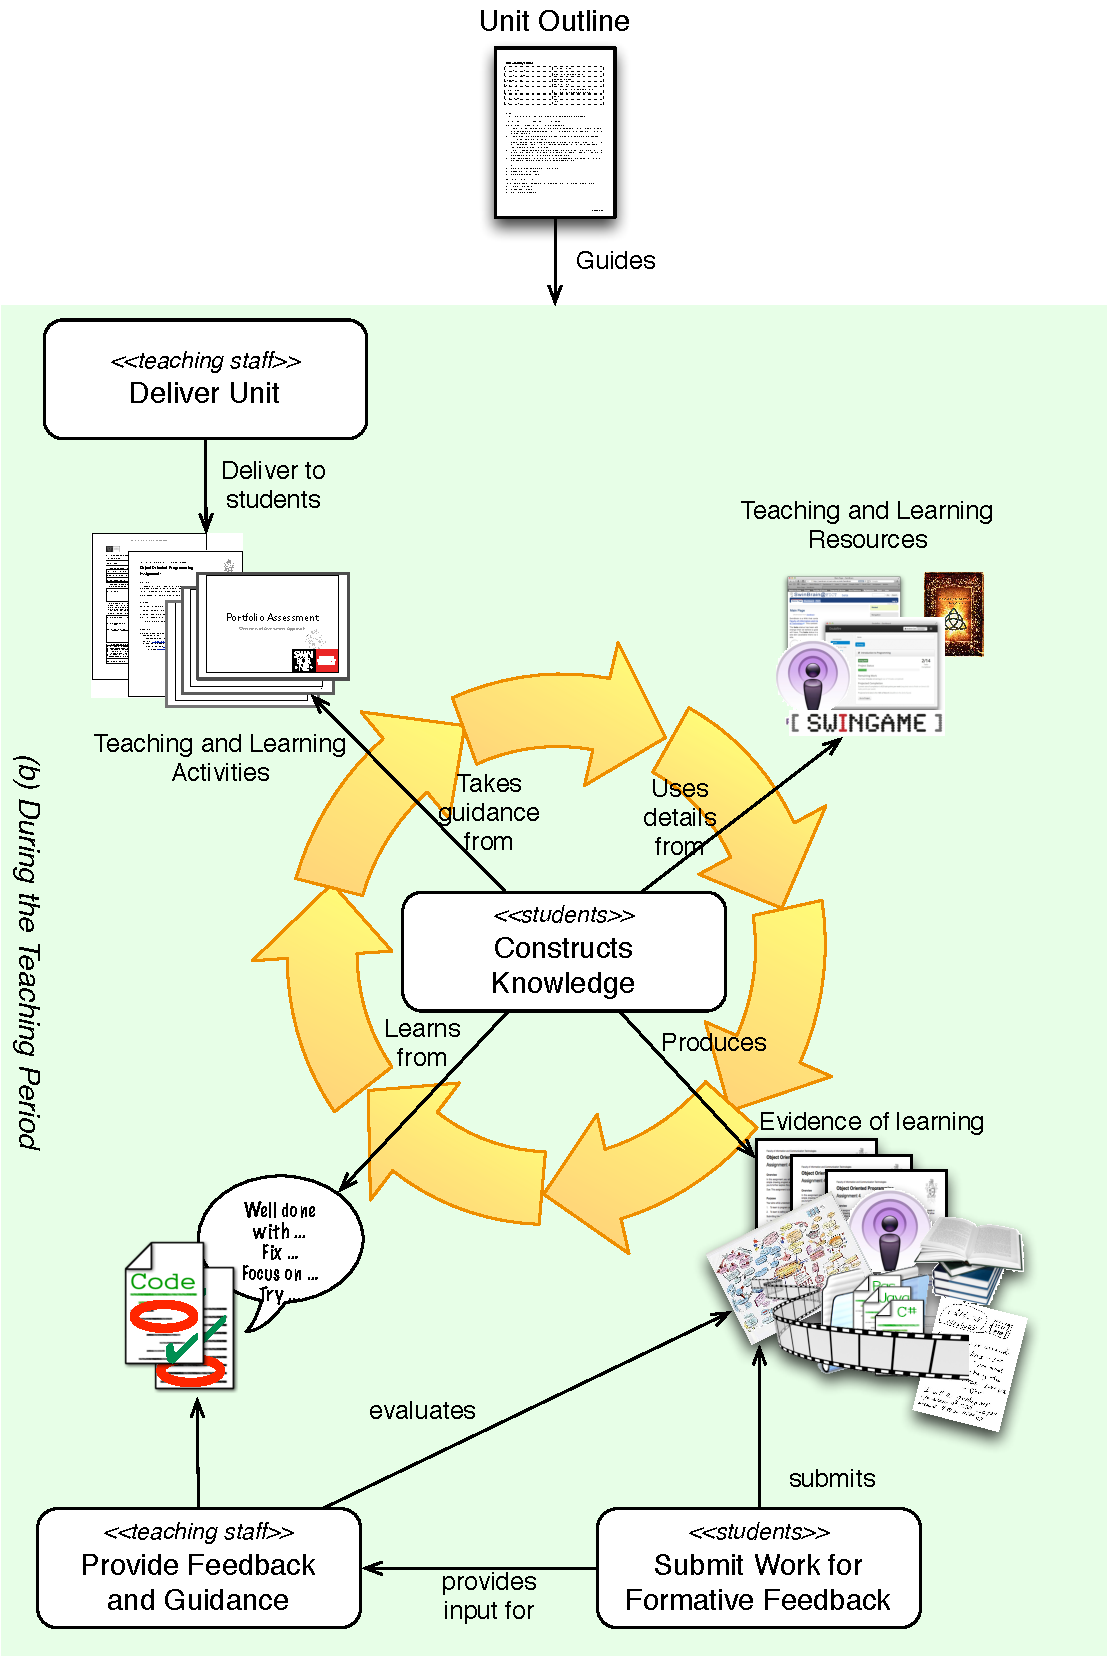
\includegraphics[width=0.9\textwidth]{DeliverUnit}
	\caption{Iterative nature of the delivery process}
	\label{fig:deliver_unit}
\end{figure}


\fref{fig:deliver_unit} illustrates the iterative delivery process at the heart of the model presented. The process centres on the students construction of knowledge, which draws up the teaching and learning activities and resources. This active process of learning generates pieces of work that the student submits for formative feedback. The teaching staff evaluate the evidence presented, trying to identify issues with the students current mental models, and provide formative feedback to the student. This feedback helps inform the student of their progress, and provides them with tasks they can act up thereby ensuring we close the loop.

All of these processes occur on a weekly basis, with rapid iteration ensuring feedback is timely and gives students the best chance of addressing misconceptions before the end of the teaching period. Each week, students will attend lectures which guide them in relation to key aspects and motivations. Undertake set tasks from tutorial handouts, while drawing upon teaching and learning resources for required details. Produce work and submit for feedback. Receive feedback and a list of changes required to meet the expected standard.

For any one topic, this iterative process may take a couple of iterations before the student is successful in getting the work signed off. \fref{fig:construct_knowledge} is an illustration shown to students to indicate the iterative nature of the submission process. The highly connected nature of the topics in introductory programming means that it is critical students understand earlier topics before they move on. Work that is submitted is not seen as complete until it demonstrates certain levels of understanding. While this is not the case, students need to correct and resubmit the work.

\begin{figure}[p]
	\centering
	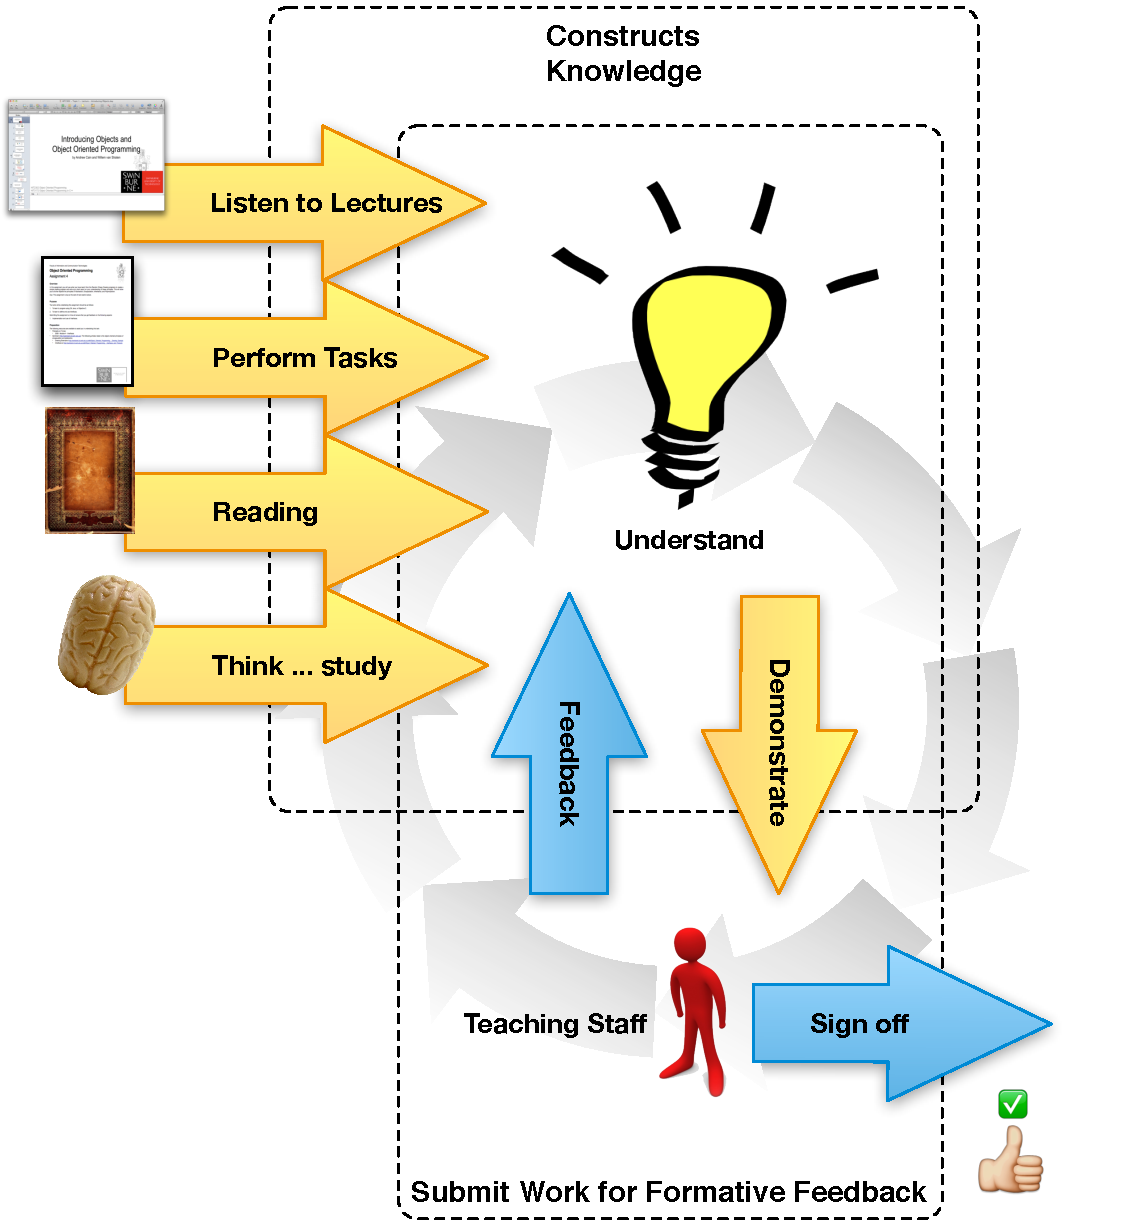
\includegraphics[width=0.9\textwidth]{ConstructKnowledge}
	\caption{Iterative process students undertake to get work signed off.}
	\label{fig:construct_knowledge}
\end{figure}

Requiring students to resubmit work ensures that no topic is half done. This focus on quality, and depth of understanding, helps communicate the high standards expected of students, \pref{itm:expectations}. Students are expected to submit some work for assessment each week. To enable fast turn around, this work is required in hard copy at the start of each week's lecture. This work is then evaluated by the teaching staff \emph{before} that week's tutorial classes. In the tutorial classes the work is returned to students, and the teaching staff briefly discuss progress with each student and the aspects of their work they can improve upon. This dialogue focuses on the students understanding, and their demonstration thereof.

The following principles were developed and used to guide the planning and delivery of teaching and learning activities:

\begin{itemize}
  \item Provide opportunities through activity design to actively engage students -- \emph{it is what the student does that counts}.  
  \item Relate all activities to the objectives, providing students with opportunities to create evidence for their portfolio.
  \item Use ungraded formative feedback to aid knowledge construction, with preference for small, frequent guidance.
\end{itemize}

% subsubsection deliver_unit (end)

\subsubsection{Construction, Submission, and Assessment of Portfolios} % (fold)
\label{ssub:construction_submission_and_assessment_of_portfolios}

The final phase of the process is the development and submission of portfolios by students, and assessment by staff. This process uses the intended learning outcomes and assessment criteria from the Unit Outline to determine what needs to be demonstrated and assessed. \fref{fig:portfolio_processes} illustrates the processes for portfolio construction by students, and assessment by staff. Students construct their portfolios from work completed during the teaching period. This work can incorporate feedback received, enabling students to showing off their best work and providing them with encouragement to act upon the feedback. \fref{fig:portfolio_pieces} shows an illustration used to explain the portfolio construction process to students. 

In preparing the portfolio, students must demonstrate that they have met all of the unit's intended learning outcomes. This alignment is documented by students in a \emph{Learning Summary Report}. The Learning Summary report starts with a self assessment, in which the student indicates which grade they are \emph{applying} for with this portfolio. The following sections provide the justifications for why the student should be awarded this grade. Students are required to list the pieces of work they have includes, and then explain how these pieces demonstrate that the student has attained all intended learning outcomes. The report ends with a reflection in which the student is encouraged to reflect upon the significance of what they have learnt, as well as on the process of learning itself. This learning summary report is then combined with the pieces of work, printed, bound and submitted for assessment.

\begin{figure}[p]
	\centering
	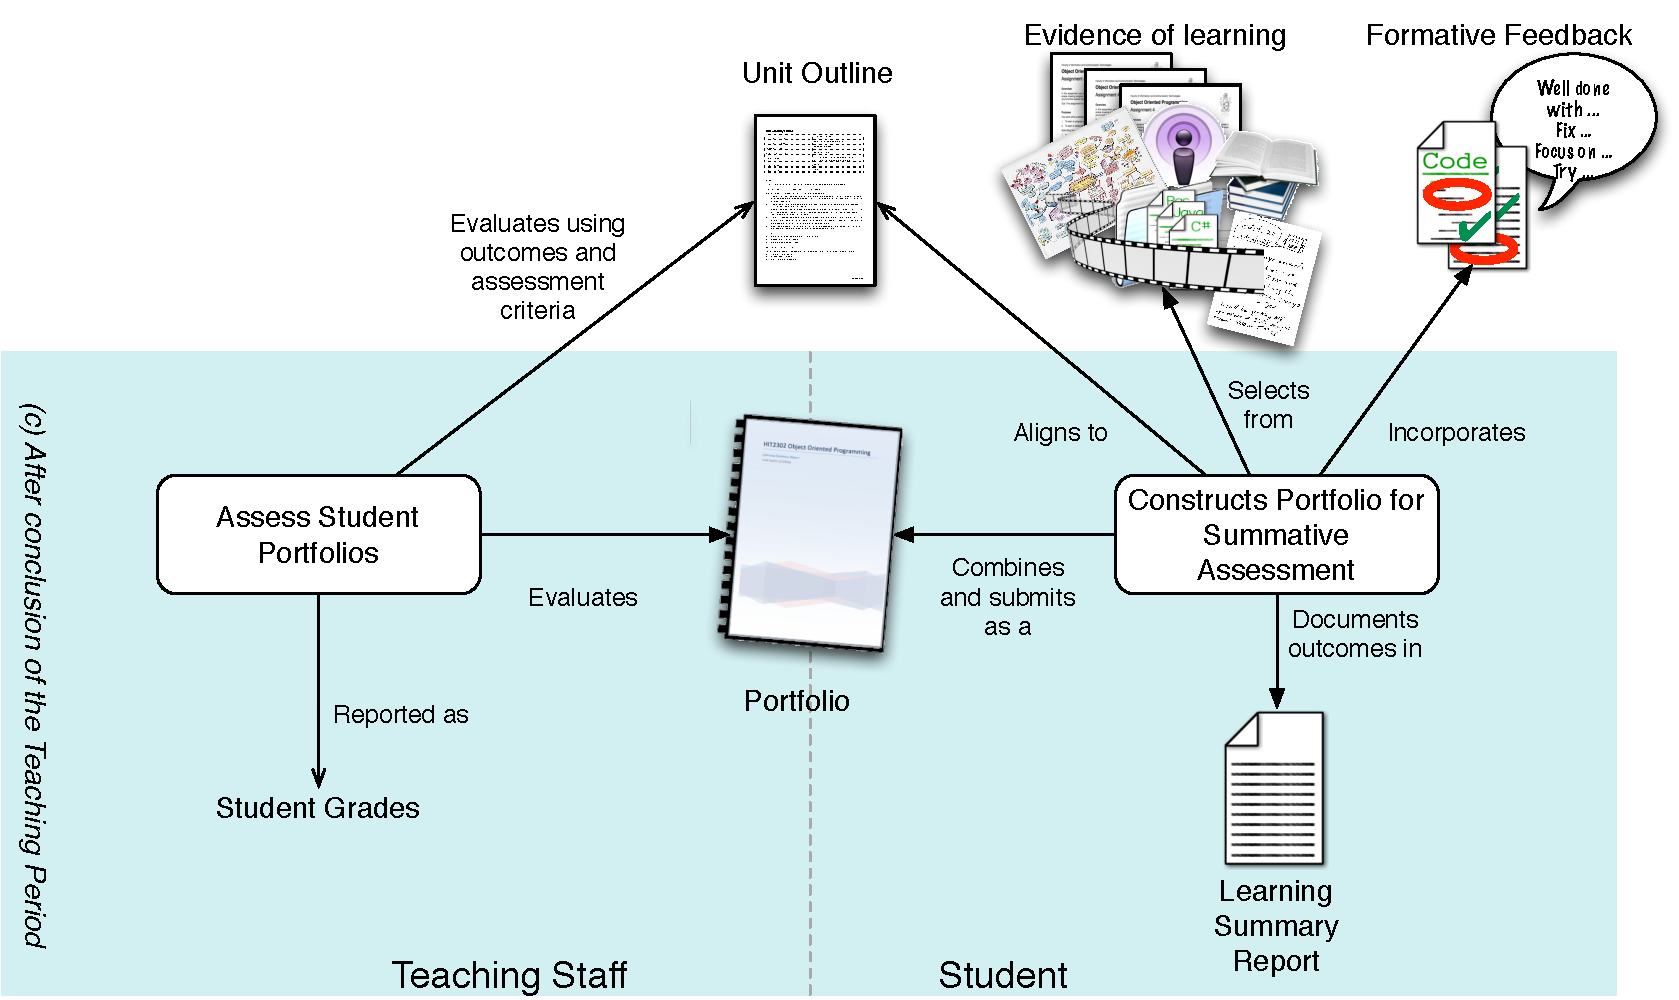
\includegraphics[width=\textwidth]{PortfolioConstructionAssessment}
	\caption{Processes of constructing, submitting, and assessment portfolios.}
	\label{fig:portfolio_processes}
\end{figure}

\begin{figure}[p]
	\centering
	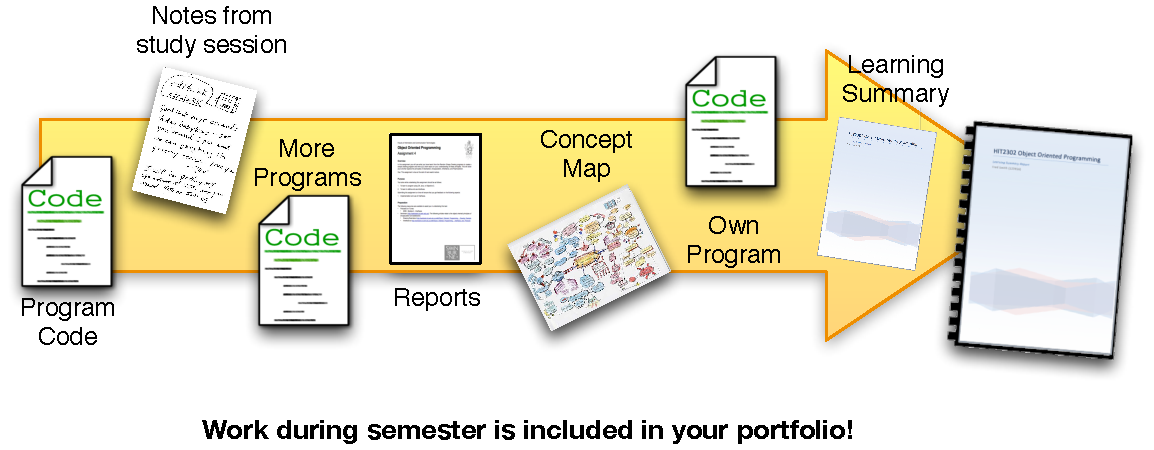
\includegraphics[width=0.9\textwidth]{PortfolioPieces}
	\caption{Illustration show to students to highlight the process of constructing their portfolio.}
	\label{fig:portfolio_pieces}
\end{figure}

The submission process differs based upon the grade students are aiming for in their portfolios. Students aiming for a pass or credit grade submit their portfolio by a set date in the examination period. These portfolios contain primarily work set out in the teaching and learning activities, and will have been checked already by teaching staff throughout the teaching period as part of the formative feedback process. Students aiming for Distinction or High Distinction are required to present their portfolio at an interview. In this interview students outline their custom work, and discuss how this relates to the unit's intended learning outcomes. The interviews are informal and encourage students to elaborate on what they have achieved.

Based on our experience we suggest the following principles be used to guide the creation and assessment activities of portfolios:
\begin{itemize}[noitemsep,nolistsep]
  \item Encourage unique, diverse, concise, and strongly aligned evidence.
  \item Motivate students to include evidence of learning from formative experience.
  \item Accurately and consistently follow the terms of the assessment criteria, as this is the \emph{contract} the students work towards.
  \item Require students to reflect on their learning, and the evidence in their portfolio, with respect to the intended learning outcomes of the unit and the assessment criteria.
  \item Use an interview, or hurdle test, to check minimal pass criteria in an invigilated manner. Where tests are used they need only distinguish between pass and fail, and do not need to address higher grades. 
\end{itemize}

% subsubsection construction_submission_and_assessment_of_portfolios (end)

\subsection{Addressing Plagiarism} % (fold)
\label{sub:addressing_plagiarism}

While embodying a predominantly Theory Y atmosphere, this model aims to minimise plagiarism through a number of factors.
\begin{itemize}[noitemsep,nolistsep]
	\item Formative assessment does not punish students for misunderstandings, in fact it actively encourages student to highlight their issues so that we can provide valuable feedback. 
	\item Weekly interactions between students and teaching staff provide an opportunity to verify understanding of the submitted work. For work to be signed off students need to be able to discuss the work with their tutors in class.
	\item A number of hurdle tests were included in the teaching and learning activities, the last of which had to be passed under examination conditions.
	\item Higher grades required an interview in which students elaborated on their work. This required the discussion of specific details that would be hard to fabricate.
\end{itemize}

Many of these aspects are primarily included for other purposes, only the hurdle tests are provided primarily for plagiarism prevention. Unlike standard examinations, these tests aim only to assess \emph{core} aspects of the unit that all students should be able to perform without issues. \fref{fig:tests} shows an illustration used to describe the tests to the students.

\begin{figure}[htbp]
	\centering
	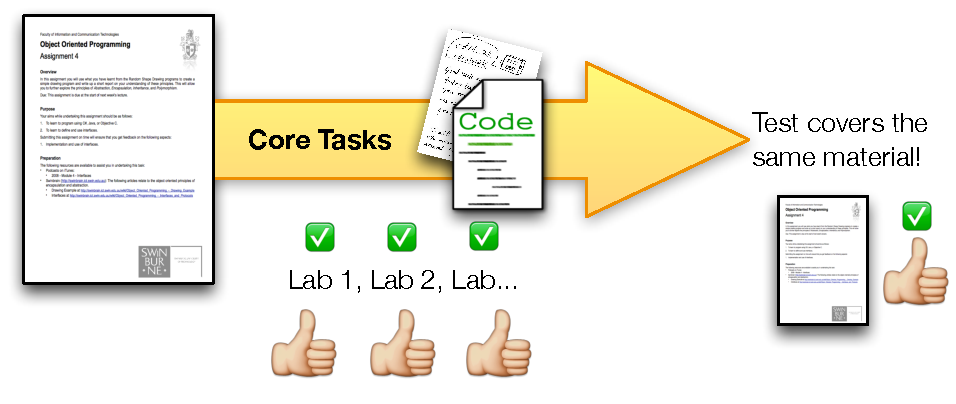
\includegraphics[width=\textwidth]{Tests}
	\caption{Tests cover aspects already presented in the tests, helping verify students completed the work themselves.}
	\label{fig:tests}
\end{figure}

As the tests only assess core competencies, the tests are marked to a high standard. Students can be awarded one of three grades: pass, fix or redo. The pass grade requires the large majority of the test to be correct. Small issues like minor syntax errors, or other small mistakes can be overlooked, but as a majority the work must demonstrate good mastery of the topics covered. Fix grades indicate some larger issues are present, but nothing critical and the work still demonstrates a sufficient mastery of the content. For both pass and fix grades, students are expected to correct all issues in their test and include the corrected versions in their portfolios. 

Students who demonstrate less than fix standard tests must redo the test. To be awarded this grade the student's test would have to indicate some critical misconceptions, or large gaps in their knowledge. It is important to note that this does not represent getting less than 50\%, or some other arbitrary percentage, of available marks. The work is assessed qualitatively, with teaching staff making expert judgements about the levels being demonstrated. The response to even a single question could demonstrate critical misunderstandings.

Students must include the tests in their portfolios, and the last test had to be passed in examination conditions. All tests also perform a formative role, with students needed to correct any issues themselves and resubmit the work, with the test only being signed off when students have been able to address it to the required standard.

Through a combination of weekly formative feedback, hurdle tests and interviews for higher grades, the model should help address issues of plagiarism without unduly emphasising punitive aspects. This is in keeping with the \pref{itm:theory_y} from \cref{cha:guiding_principles}.

% subsection addressing_plagiarism (end)

\section{Summary} % (fold)
\label{sec:summary}

This chapter has outlined an overall strategy for teaching introductory programming with portfolio assessment based on an objects-later approach. Using the principles from \cref{cha:guiding_principles}, a model for the development of constructively aligned units was presented. \cref{cha:example_impl} continues this work by demonstrating the application of this model in the creation and delivery of two introductory programming units.

% section summary (end)

% chapter approaching_constructive_alignment_with_portfolio_assessment (end)